\documentclass[10pt,a4paper]{article}
\usepackage[
nochapters, % Turn off chapters since this is an article        
beramono, % Use the Bera Mono font for monospaced text (\texttt)
eulermath,% Use the Euler font for mathematics
pdfspacing, % Makes use of pdftex’ letter spacing capabilities via the microtype package
dottedtoc % Dotted lines leading to the page numbers in the table of contents
]{classicthesis} 
\usepackage[a4paper,top=2.5cm,bottom=3cm,left=2.8cm,right=2.8cm,bindingoffset=0mm]{geometry}
\usepackage[utf8]{inputenc}
\usepackage[T1]{fontenc}
\usepackage[italian]{babel}
\usepackage{amsmath}
\usepackage{amsfonts}
\usepackage{amssymb}
\usepackage{makeidx}
\usepackage{placeins}
\usepackage{graphicx}
\makeatother
\author{Fabio Prestipino}
\title{Guida ROOT}
\begin{document}
	
	\maketitle
	\tableofcontents
	\newpage
Per istogrammi saranno convenzionalemnte usati i nomi h, h0, h1,...; per le funzioni f, f0, f1, f2,...; per le funzioni di fit fit, fit1,...; per i grafici g, g1, g2, ...; l per le legende e c per le canvas
\section{Introduzione ed informazioni generali utili}
ROOT è un linguaggio ad oggetti sviluppato dal CERN basato su C++ utile per l'analisi ed elaborazione di grandi moli di dati. Ogni istogramma, grafico, funzione (...) che creiamo è un oggetto con delle sue opzioni e funzioni (funzioni membro). Una proprietà fondamentale è l'ereditarietà: tutte le classi sono figlie di una classe di base (TObject) da cui discendono le altre; ogni classe figlia eredita le funzioni membro di quelle precedenti. Il tipo degli oggetti comincia sempre con la lettera T, seguita da altre lettere che specificano le caratteristiche dell'oggetto. Di seguito riporto alcune informazioni di base in ordine casuale:
\begin{itemize}
\item I tipi base di ROOT hanno nomi leggermente diversi da quelli di c++: \(Int\_t\), \(Float\_t\), \(Double\_t\), TString...\\
\item Per stampare a schermo basta usare i comandi di C++. Ad esempio:\\\\
Double\_t a;\\
cout<< "Scritta" << a;\\
\item Per accedere ai file di ROOT il codice da scrivere sulla barra di comando è\\\\
TBrowser b;\\
\item Per usare funzioni matematiche è possibile utilizzare la libreria di Root "TMath", ad esempio:\\\\
TMath::Sin(TMath::Pi()/2.) = 0\\\\ 
\item Per salvare un oggetto (grafico, istogramma,...) come file ROOT bisogna aprire un file ROOT scriverci l'oggetto dentro e chiuderlo:\\\\
TFile *nome = new TFile(“nome\_file.root”,”RECREATE”);\\
nome\_oggetto -> Write();\\
nome -> Close();\\
\item Per accedere a file di dati (che dovrà essere nella stessa cartella della macro) si usa la funzione di C++ fstream(); in ordine bisogna creare un oggetto file, aprire quello desiderato, accedervi e chiuderlo. In ordine:\\\\
 fstream nome;\\
 nome.open("nome\_file.txt");\\
 nome >> x;\\
 nome.close();\\\\
\end{itemize}
\subsection{Come interfacciarsi}
Esistono 3 modi di interfacciarsi a ROOT: 
\begin{itemize}
\item \textbf{Command line}\\
Utile per comandi di base, è più flessibile delle macro (ad esempio non serve il ;). Per accedere al terminale direttamente da ROOT basta scrivere i normali comandi del terminale preceduti da un ".! ". Per uscire da ROOT basta scrivere sulla barra di comando .q oppure se non funziona .qqqqq...
\item \textbf{Macros}\\
Esistono due metodi: uno è quello \textbf{interpretato}. Un file scritto in un editor di testo che poi viene eseguito su ROOT. Una macro si presenta come una normale funzione di c++, può prendere parametri che poi vengono usati al suo interno e si possono creare altre funzioni all'interno. Di seguito un esempio di macro vuota\\\\
void nome(parametro1, parametro 2, ...)\{\}\\\\
\'{E} inoltre possibile far girare una macro in due modi diversi: o facciamo partire tutta la macro, eseguendo così tutte le funzioni al suo interno, con il comando\\\\
.c name.C\\\\
Se la macro è formata da una singola funzione si può usare direttamente il comando\\\\
.x myMacro.C\\\\
per far partire la funzione.
\'E anche possibile caricare le funzioni della macro in memoria con il comando\\\\
.L name.C\\\\
per poi chiamare le funzioni singolarmente, ad esempio:\\\\
funz1();\\\\
IN MODALITA INTERPRETATA NON SI DEVONO INCLUDERE I PACCHETTI ROOT.\\
Un metodo alternativo è quello \textbf{compilato}: si includono tutti gli oggetti di ROOT necessari e si scrive una macro (che si presenta sempre come una o più funzioni C++) che dovrà essere compilata esternamente (ad esempio con un classico g++) o direttamente in ROOT con il comando \\\\
.L myMacro.C+\\\\
(si faccia attenzione all'aggiunta del "+" a fine comando) per poi eseguirla come una normale funzione\\\\
myMacro()\\\\
IMPORTANTE: LE MACROS DEVONO STARE NELLA CARTELLA IN CUI VIENE APERTO ROOT
\item \textbf{Finestra grafica (GUI)}\\
Per curare l'estetica dei grafici è possibile sfruttare l'interfaccia grafica, più intuitiva. Per far comparire le opzioni della finestra bisogna cliccare su "view" e spuntare "editor", "toolbar" ed "event statusbar". 
\end{itemize}
\section{ROOT Files}
Esistono file di tipo .root all'interno dei quali si possono scrivere (e quindi salvare in memoria per poi poterli leggere in altri files) oggetti ROOT come funzioni e istogrammi o oggetti user-defined (trattati in seguito). I file .root sono gestiti con la classe TFile, l'idea è che si crea un oggetto di tipo TFile che si inizializza o assegnandogli un file .root preesistente o generandone uno ex-novo, in questo modo potremo aprire, leggere e scrivere quel file per poi salvarlo e chiuderlo.\\
Possiamo inizializzare un file in vari modi, a seconda di ciò che vogliamo fare con questo: possiamo aprirlo "in lettura" (se non specifichiamo opzioni), "in scrittura" (con opzione "RECREATE" crea un nuovo file e se già esisteva lo sovrascrive, "NEW" e "CREATE" creano un nuovo file e se già esiste non fanno niente), in "modifica" (l'opzione "UPDATE" apre un file che, se già esistente, può essere modificato e se non esistente viene creato). La sintassi è:\\\\
TFile *file = new TFile(“example.root”,“OPZIONE");\\\\
Per listare il contenuto del file esiste il metodo ls:\\\\
file->ls();\\\\
Una volta aperto il file è possibile accedere ai suoi elementi con il metodo Get\\\\
TH1F *histo=(TH1F*)file->Get(“histo”);\\\\
Per scrivere un singolo oggetto sul file si usa il metodo:\\\\
object -> Write();\\\\
Se invece si vogliono scrivere sul file tutti gli oggetti nella memoria corrente (ovvero inizializzati nel file fino ad ora):\\\\
file->Write();\\\\
Per chiudereilfile root siusailmetodo Close:\\\\
file->Close();\\\\
\subsection{Decoupling objects}
Normalmente gli oggetti di un file si dicono "coupled" con il file, cioè spariscono dalla canvas una volta chiuso il file. Per evitare che ciò avvenga bisogna effettuare il "decouple" con uno dei tre seguenti metodi :\\\\
object->AddDirectory(kFALSE); (statico)\\
object->SetDirectory(kFALSE); (non statico)\\
object->DrawCopy() (non statico)

\section{Istogrammi}
\subsection{Inizializzare e riempire un'istogramma}
Il tipo degli istogrammi è formato da 4 lettere: la T(come per tutti gli oggetti), una H di "histogram", un numero che indica il numero di dimensioni dell'istogramma e un'ultima lettera che può essere I (int), F (float), D (double) che indica il modo in cui vengono rappresentati i dati nell'istogramma. Un'istogramma di base sarà, ad esempio, del tipo "TH1F".\\
\'{E} raccomandato dichiarare (costruire) un'istogramma usando i puntatori, di seguito un format di dichiarazione di un'istogramma unidimensionale:\\\\
TH1F *h = new TH1F("h", "titolo", n-bin, \(x_{min}\), \(x_{max}\)); \\\\
Dove n-bin è il numero di bin che vogliamo nell'istogramma ed \(x_{min}\), \(x_{max}\) il range entro cui vogliamo vedere l'istogramma. Possiamo inizializzare anche un'istogramma senza passare alcun parametro\\\\
TH1F *h = new TH1F(); \\\\
Oppure con il copy constructor, passando by pointer un altro istogramma\\\\
TH1F *h1 = new TH1F("h1", "histo1", n-bin, \(x_{min}\), \(x_{max}\));\\\\
TH1F *h2 =  new TH1F(*h1);\\\\
 Per aggiungere punti ad un'istogramma unidimensionale:\\\\
h -> Fill(x);\\\\
la funzione Fill può accettare anche un secondo paramentro che permette di aggiungere in una volta tante entrate uguali:\\\\
h -> Fill(x, 8);\\\\
aggiunge 8 entrate x all'istogramma.\\
Se invece volessimo più dimensioni:\\\\
TH2F *h = new TH2F("h", "titolo", \(n_x-bin\), \(x_{min}\), \(x_{max}\), \(n_y-bin\), \(y_{min}\), \(y_{max}\)); \\\\
Per aggiungere punti in un'istogramma bidimenzionale:\\\\
h -> Fill(x,y);\\\\
\'{E} inoltre possibile fare le proiezioni degli istogrammi multidimenzionali sui singoli assi:\\\\
h1 -> ProjectionX();\\
h2 -> ProjectionY();\\\\
che crea un'istogramma già riempito.\\

\subsection{Inserire dati da file}
\'{E} possibile riempire un'istogramma sfruttando i dati di un file di testo (che dovrà essere nella stessa cartella della macro). Innanzitutto bisogna costruire l'oggetto file\\\\
fstream nome;\\\\
poi bisogna aprire il file desiderato\\\\
nome.open("nome\_file.txt")\\\\
infine con un ciclo aggiungiamo i dati del file fin quando questo non finisce:\\\\
Float\_t x;\\
while(1)\{\\
	nome >> x;\\
	h -> Fill(x);\\
	if(!nome.good()) break;\\
\}\\
nome.close();\\\\

Dove "nome" è il nome dell'oggetto-file che inizializziamo e a cui assegniamo il file di testo che si desidera aprire, che si chiama "nome\_file.txt". Il metodo nome.good() dice se il file è concluso o meno. Nell'ultima riga è stato chiuso il file. 
\subsection{Metodi utili istogrammi}
Di seguito sono riportati i metodi più importanti per gli istogrammi
\begin{itemize}
	\item h ->GetXaxis()->SetTitle("titolo");
	setta il titolo dell'asse
	\item h -> SetMarkerStyle(numero);\\
	assegna uno stile al marker
	\item h -> SetMarkerSize(numero);\\
	assegna una grandezza al marker
	\item h -> GetBinError(nbin);\\
	prende l'errore di un bin
	\item h -> GetBinContent(nbin);
	prende il numero di entrate nel bin
	\item h -> GetBinContent(0);
	prende il numero di entrate in underflow
	\item h -> GetBinContent(nbin+1);
	prende il numero di entrate in overflow
	\item h -> GetEntries();\\
	prende il numero di entrate totali
	\item h -> SetBinContent(ibin,val);\\
	assegna al contenuto del bin un valore val
	\item h -> GetMean();\\
	calcola la media
	\item h -> GetRMSError();\\
	calcola l'errore sulla media
	\item h -> GetRMS();\\
	calcola la deviazione standard
	\item h -> GetMeanError();\\
	calcola l'errore sulla deviazione standard
	\item h -> GetMaximum();\\
	prende il bin con numero massimo di entrate
	\item h -> GetMaximumbin();\\
	prende il numero del bin con numero massimo di entrate
	\item h -> GetBinCenter();\\
	prende il centro del bin
	\item h -> GetIntegral();\\
	restituisce un'array dei conteggi cumulativi 
	\item h -> Integral();\\
	calcola l'integrale nel range
\end{itemize}
\subsection{Operazioni fra istogrammi}
Si possono usare metodi dedicati della classe per effettuare operazioni tra oggetti di ROOT; le operazioni utili sono somma (talvolta sottrazione) e divisione. Seguiamo gli step necessari:
\begin{enumerate}
	\item Creare e riempire gli istogrammi con cui operare
	\item Creare l'istogramma risultato, inizialmente vuoto, passando come parametro il primo istogramma con cui si vole operare. Per la divisione:\\\\
	TH1F *hdiv = new TH1F(*h1);\\
	hdiv -> Divide(h1,h2,1,1);\\\\
	Per la somma:\\\\
	TH1F *hsum =new TH1F(*h1);\\
	hsum -> Add(h1,h2,1,1);\\\\
	Per la sottrazione si usa la stessa sintassi dell'addizione ma con un "-1" al posto del secondo "1".\\
	Infine, per avere incertezze corrette sugli istogrammi risultato, è necessario usare il metodo Sumw2() prima di effettuare la somma prima di riempire l'istogramma:\\\\
	h1 -> Sumw2();\\
	h2-> Sumw2();\\
\end{enumerate}

\section{Grafici}
Un grafico rappresenta una serie di N coppie di due variabili (x, y). Esistono due tipi di grafici: quello semplice TGraph e quello in cui è possibile includere anche gli errori nel grafico TGraphErrors. 
\subsection{Costruttore di TGraph}
Il costruttore di TGraph di base genera semplicemente un grafico di n punti presi da due array (una che contiene tutte le x ed una le y). \\\\
TGraph *g = new TGraph (n\_punti, *nome\_arrayx, *nome\_arrayy)\\\\
dove le array sono passate con il puntatore (nome preceduto da asterisco).\\
Un altro importante costruttore di TGraph è quello che prende i punti da un file esterno, la sua inizializzazione è \\\\
TGraph *g = new TGraph (*filename, *format="\%lg \%lg") \\\\
dove il format fornisce informazioni al programma su come prendere i dati dal file di testo, in questo caso "\%lg \%lg" dice di prendere le prime due colonne di numeri double separate da un blank delimiter (spazio bianco). Se si volesse saltare una colonna basta aggiungere un'asterisco: "\%lg \%*lg \%lg". Se si inseriscono più di due colonne (al minimo devono essere due), si crea un grafico a più dimensioni. Se il file di dati è formato solamente dal numero di colonne necessario e non bisogna escludere nessuna colonna è possibile inizializzare il grafico semplicemente come 
\\\\
TGraph *g = new TGraph (*filename) \\\\
\subsection{Costruttore di TGraphErrors}
TGraphErrors si inizializza alo stesso modo di tGraph ma bisogna aggiungere l'informazione sugli errori. Il primo metodo diventa:\\\\
TGraphErrors *g = new TGraphErrors (n\_punti, *nome\_arrayx, *nome\_arrayy, *nome\_errx, *nome\_erry)\\\\
dove err\_x ed err\_y sono array conteneti gli errori per ogni coordinata di ogni punto del grafico. Per specificare che non si vogliono inserire errori in una variabile, ad esempio la x, basta sostituire uno 0 a *nome\_errx\\\\
TGraphErrors *g =new TGraphErrors(n\_punti, *nome\_arrayx, *nome\_arrayy, 0, *nome\_erry);\\\\
Il secondo metodo invece diventa: \\\\
TGraphErrors *g = new TGraphErrors (*filename, *format="\%lg \%lg \%lg") )\\\\
dove questa volta il numero minimo di colonne è 3. A rigore dovrebbe essere 4 (le prime due sono le misure di x ed y e le seconde i relativi errori) ma se sono solo 3 si interpreta l'ultima come gli errori sia sulla x che sulla y. Anche in questo caso se il file dei dati è formato solamente dalle colonne necessarie e non serve escludere colonne la sintassi si riduce a\\\\
TGraphErrors *nome = new TGraph (*filename)\\\\
ATTENZIONE: LA VIRGOLA NON \'{E} LETTA COME SEPARATORE DECIMALE, SERVE IL PUNTO. 
\subsection{Metodi per grafici}
Di seguito i principali metodi dei grafici
\begin{itemize}
	\item g -> SetTitle(“Titolo; Titolo\_asseX; Titolo\_asseY");
	\item g -> SetMarkerStyle(kOpenCircle);
	\item g -> SetMarkerStyle(numero);
	\item g -> SetMarkerColor(kBlue);
	\item g -> SetLineWidth(2);
	\item g -> SetLineColor(kBlue);
	\item g -> GetPoint(i, x, y);
	prende l’iesimo punto del grafico
	\item g -> GetX ()/GetY ();
	ritorna un puntatore ad un'array con tutte le coordinate x (o y). 
	\item g -> GetN();
	ritorna il numero di punti nel grafico
	\item g -> Integral();
	calcola l'integrale da inizio a fine grafico
	\item g -> AddPoint(x,y);
	aggiunge un punto di coordinate x, y al grafico
	\item g -> SetPoint (i,x,y);
	sovrascrive il valore dell'iesimo punto del grafico
	\item g -> GetCorrelationFactor();
	calcola il coefficiente di correlazione lineare fra i punti
	\item g -> GetCovariance();
	calcola la covarianza fra i punti
	\item g -> Fit( "formula");
	effettua un fit a partire da una formula scritta come una stringa; deve essere scritta nella forma [0]+x*[1]
	\item g -> Fit(nome\_funzione);
	effettua un fit a partire da una funzione precedentemente definita
\end{itemize}
(kOpenCircle e kBlue sono codici predefiniti in ROOT, li ho messi per esempio)

\section{Variabili globali}
I puntatori globali puntano ad informazioni generali sul file in uso sono principalmente 4:
\begin{itemize}
	\item gROOT\\
	informazione globale relativa alla sessione corrente con cui si può accedere a qualunque oggetto in essa
	\item gFile\\
	puntatore al root file corrente
	\item gStyle\\
	puntatore alle funzionalità di stile
	\item gRandom\\
	puntatore al generatore di numeri casuale, che verrà approfondito nella sezione \ref{sec:montecarlo}.
\end{itemize}
Di solito si crea una funzione prima di cominciare la funzione principale della macro in cui si settano le variabili globali, ad esempio
void SetStyle() \{
	gROOT->SetStyle("Plain");
	gStyle->SetPalette(57);
	gStyle->SetOptTitle(0);
\}
\section{Funzioni di ROOT}
Le funzioni sono oggetti che possono essere definite dall'utente o prese dagli oggetti di ROOT (ad esempio gaussiana, esponenziale, polinomiale,...). Le funzioni in generale sono di tipo TF seguito da un numero che ne indica la dimensione; ad esempio quelle ad una variabile sono contraddistinte dall'"1" alla fine del nome del tipo.
\subsection{Inizializzazione e funzioni utili}
Le funzioni definite dal'utente possono essere dichiarate in tre modi:
\begin{itemize}
	\item Stringa di caratteri nel costruttore (riconosce le funzioni della libreria cmath)\\\\
	TF1 *f = new TF1("f", "sin(x)/x“, x\_iniziale, x\_finale);\\\\
	\'{E} inoltre possibile usare e modificare funzioni già esistenti\\\\
	TF1 *f1 = new TF1("f1", "f*x", x\_iniziale, x\_finale);\\\\
	\item Stringa di caratteri con parametri da inizializzare\\\\
	TF1 *f = new TF1 ("f",“ [0]*x*sin([1]*x)",x\_iniziale, x\_finale);\\\\
	dove i numeri fra parentesi quadre sono parametri liberi che possono essere definiti con\\\\
	f -> SetParameter(numero\_parametro, valore);\\\\
	dove "numero\_parametro" è il numero del parametro che vogliamo definire (nel nostro esempio o 0 o 1) e "valore" è il valore che vogliamo dare a quel parametro.\\
	\'{E} del tutto equivalente inizializzare la funzione specificando nel costruttore il numero di parametri:\\\\
	TF1 *f = new TF1 ("f","funzione",x\_iniziale, x\_finale, numero\_parametri);\\\\
	In questo caso sarà possibile definire tutti i parametri in una volta con\\\\
	f -> SetParameters(valore1,valore2, ...);\\
	\item Definita in una macro\\
	Si usa la sintassi di C++, ad esempio:\\\\
	MyFunction(Double\_t *x, Double\_t *par)\{
		 Float\_txx =x[0];\\
		 Double\_t val= TMath::Abs(par[0]*sin(par[1]*xx)/xx);\\
		 return val;
		 \};\\
	e poi si inizializza\\\\
	TF1* f = new TF1("f", "MyFunction(x, par)", 0, 10);
\end{itemize}
Esistono anche funzioni built-in ROOT che si dichiarano così:\\\\
TF1 *f = new TF1("f", "funzione");\\\\
dove "funzione" indica il nome della funzione di ROOT, alcuni esempi sono: 
\begin{itemize}
	\item poln: [0] + [1]*x + [2]*x2 +...
	\item gaus: \ [0]*exp(-0.5 *(x-[1])/[2])\^2\\\\
	dove i parametri rappresentano:\\\\
	\ [0] = ampiezza massima in corrispondenza della media\\
	\ [1] = media\\
	\ [2] = sigma\\\\
	\item expo: exp([0]+[1]*x)\\\\
	dove i parametri rappresentano:\\\\
	\ [0] = ampiezza\\
	\ [1] = media\\
	\item gausn: [0]*exp(-0.5*((x-[1])/[2])\^2)/([2] *sqrt(2PI))
\end{itemize}
Alcuni metodi delle funzioni sono:
\begin{itemize}
	\item f -> Eval(x);\\
	valuta la funzione in quel punto
	\item f -> Integral(a, b)\\
	calcola l'integrale fra i punti a e b
	
\end{itemize}
\subsection{Fitting}
Per effettuare un fit di dati in un istogramma rispetto ad una funzione definita dall'utente bisogna:
\begin{enumerate}
	\item Creare una funzione con parametri liberi che pensiamo sia adeguata a fittare i dati\\\\
	TF1 *fit = new TF1("fit","funzione con parametri", x\_min, x\_max);\\
	\item 'E altamente consigliato (talvolta necessario se no non fitta) settare i parametri che ci aspettiamo di ottenere approssimativamente dal fit con l'apposita funzione\\\\
	fit->SetParameter(n\_parameter, value);\\\\
	\item Effettuare il fit, che non fa altro che assegnare parametri alla funzione del fit\\\\
	h -> Fit("fit");\\
	\item Possiamo prendere i parametri con la funzione:\\\\
	 fit -> GetParameter(n\_parameter);\\
	 fit -> GetParameters(nome\_array);\\\\
	 il primo metodo prende solamente l'iesimo parametro mentre il secondo crea una array con tutti i parametri.\\
\end{enumerate}
Per effettuare un fit a partire da una funzione built-in ROOT basta scrivere:\\\\
nome\_isto -> Fit(funzione);\\\\
dove al posto di funzione si può mettere il nome di una funzione built-in ROOT (linear, poln, gaus, expo, gausn...)
Di seguito altre utili funzioni membro delle funzioni fit
\begin{itemize}
	\item fit -> GetChisquare(); 
	prende il Chiquadro
	\item fit -> GetNDF();
	prende i gradi di libertà
	\item fit -> GetParError(i);
	prende l'errore dell'iesimo parametro
	\item fit -> GetParErrors(nome\_array);
	crea un'array con tutti gli errori sui parametri. Si potrebbe anche creare un'oggetto array ed assegnargli la funzione con le parentesi vuote.
\end{itemize}
\'{E} possibile fittare anche grafici grazie all'overloading della funzione Fit:\\\\
g -> Fit("nome\_funzione");\\
 \subsubsection*{Fit in sotto-range}
 Spesso capita che si voglia fittare solo una parte di grafico o istogramma. Esistono vari modi per farlo:
 \begin{itemize}
 	\item Si dichiara un range di validità (dominio) nel costruttore della funzione e poi si fitta usando l'opzione "R":\\\\
 	TF1 *f = new TF1("f", "funzione", range\_min, range\_max);\\
 	h -> Fit("f", "R");\\
 	\item Specificare come opzione di Fit il range. In questo caso la funzione si dichiara nel modo classico e per fittare si scrive:\\\\
 	h -> Fit("f", " ", " ", range\_min, range\_max); 	
 \end{itemize}
Se si specifica il range è possibile fittare utilizzando più funzioni per i diversi range. Gli step da seguire sono:
\begin{enumerate}
	\item Definire le n funzioni con cui si vuole fittare (di solito si usano le built-in come "gaus" da mettere al posto di "fi") e fare la somma:\\\\
	TF1 *f1 = new TF1(“f1", f1, range1, range2);\\
	TF1 *f2 = new TF1(“f2", f2, range3, range4);\\
	TF1 *fn = new TF1(“fn", fn, rangen-1, rangen);\\
	TF1 *ftot = new TF1("ftot","f1+f2+...+fn", range1, rangen);\\\\
	dove f1,...,fn sono le funzioni pre definite con cui si vuole fittare. 
	\item Fittare ogni sotto-range con le funzioni\\\\
	h -> Fit(f1, "R");\\
	h -> Fit(f2, "R");\\
	h -> Fit(fn, "R");\\\\
	\item Recuperare i parametri dopo il fit ad esempio in una array\\\\
	Double\_t nome\_array[numero\_parametritot];\\
	g1->GetParameters(\&nome\_array[i]);\\
	g2->GetParameters(\&nome\_array[j]);\\
	g3->GetParameters(\&nome\_array[k]);\\\\
	dove la "\&" serve perchè si passa l'array by-reference e i numeri i,, j, k indicano i parametri che si devono prendere dalle singole funzioni. 
	\item Inserire i parametri risultanti in “total” (funzione somma)\\\\
	ftot -> SetParameters(nome\_array);\\
	\item Fittare nuovamente con la funzione somma per una stima definitiva dei parametri:\\\\
	h -> Fit(total, "R")\\
	\item Estrarre risultati finali dai metodi delle funzioni fit già visti.
\end{enumerate}
\section{Classi user-defined in ROOT}
In ROOT vi sono classi predefinite come quella delle funzioni o degli istogrammi, e se volessimo usare dentro ROOT una classe user-defined, che eventualmente faccia uso di altre classi ROOT? Possiamo semplicemente implementaere una classe esternamente a ROOT (con la convenzione classica di creare un file di intestazione .h ed uno di implementazione .cpp), in questo caso dovremo includere tutti gli oggetti di ROOT necessari (per includere una classe user-defined si deve usare una macro compilata). Per compilare la classe si usa la sintassi:\\\\
gROOT->LoadMacro(“MyClass.cxx+”)\\\\
Ora possiamo usare la classe da noi definita, in altre macros (queste dovranno essere compilate dopo la claasse user-defined).\\
Per usare oggetti della nostra classe anche in file ROOT (e non solo in macros compilate) bisogna modificare il file .h della classe user-defined rendendola classe figlia (ereditarietà pubblica) di TObject, bisogna inoltre aggiungere la chiamata alla macro ClassDef(ClassName,N); bisogna modificare il file .cpp la chiamata a ClassImp(ClassName).
\begin{figure}[h!]
	\centering
	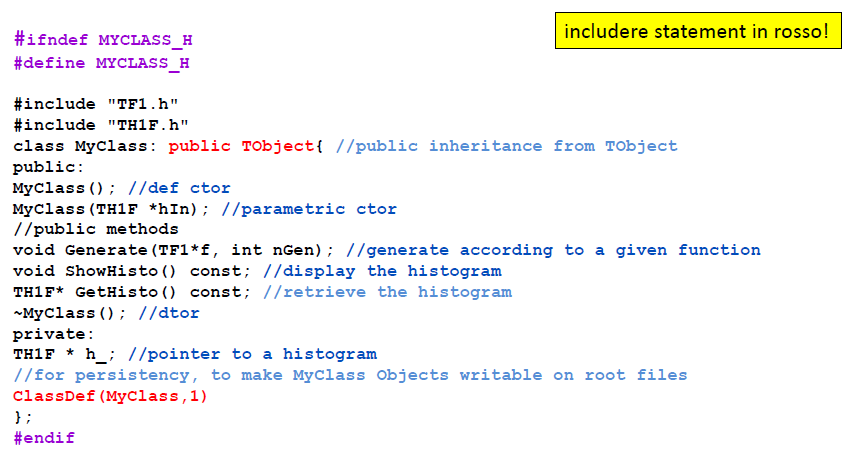
\includegraphics[width=1.\linewidth]{classi-root-1}
	\caption{Ciò che bisogna modificare alla macro (nel file .h) che definisce una classe user-defined per poter usare quella classe in un file .root}
	\label{fig:classi-root-1}
\end{figure}
\FloatBarrier
\begin{figure}[h!]
	\centering
	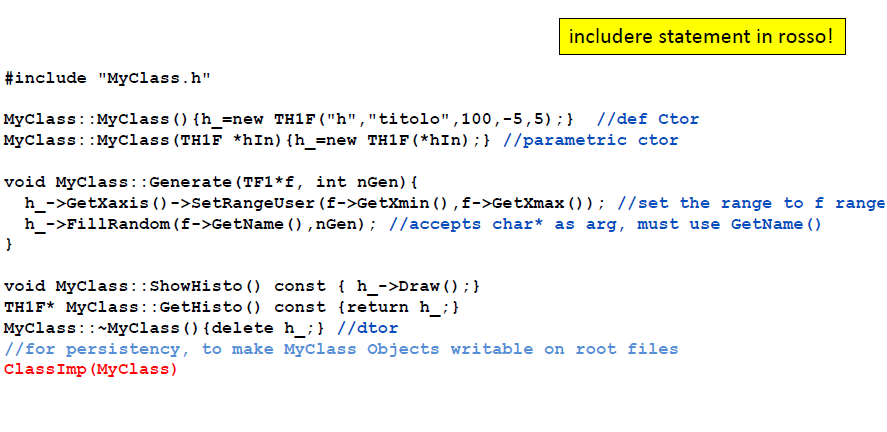
\includegraphics[width=1.\linewidth]{classi-root-2}
	\caption{Ciò che bisogna aggiungere al file .cpp che definisce la classe user-defined.}
	\label{fig:classi-root-2}
\end{figure}
\FloatBarrier
Ora possiamo scrivere l'oggetto della classe user-defined. Per leggere l'oggetto user defined scritto in un file, su un altro file, si segue il normale iter già esposto nella sezione "ROOT files.\\
Infine, per evitare di includere più volte le stesse classi user-defined si usano le inlude guards, da includere in ogni macro che usa un'oggetto user-defined:\\\\
R\_\_LOAD\_LIBRARY( MyClass\_cxx.so )\\
\section{Legenda}
La legenda è un oggetto a se stante (TLegend) che deve essere disegnato sulla canvas. Un esempio è:\\\\
TLegend *l = new TLegend(.1,.7,.3,.9,“Titolo");\\
l -> AddEntry(oggetto1, "label1");\\
l -> AddEntry(oggetto2, “label2");\\
l -> Draw("SAME");\\\\
dove i numeri nella dichiarazione di TLegend sono parametri per le dimensioni del rettangolo della legenda; AddEntry aggiunge alla legenda oggetti (quindi non solo istogrammi o grafici ma anche numeri, ad esempio il Chiquadro). 
\section{Disegnare oggetti}
\subsection{Canvas}
Per prima cosa bisogna creare una "canvas" che è l'ambiente in cui è possibile disegnare gli oggetti. Un modo base per inizializzarla è\\\\
TCanvas *c = new TCanvas();\\\\
In questo modo si crea una canvas vuota di dimensioni automatiche. \'{E} inoltre possibile specificare il nome, il titolo e le dimensioni:\\\\
TCanvas *c = new TCanvas("c", "titolo", larghezza, altezza);\\\\
Per disegnare su una canvas basta chiamare il metodo Draw() su un oggetto, che sarà disegnato automaticamente sull'ultima canvas. Se però si chiama nuovamente il Draw() su un altro oggetto questo verrà sovrascritto su quello precedente, eliminandolo. Per disegnare più oggetti su una stessa canvas bisogna dividerla in pads:\\\\
c -> Divide(larghezza1, altezza1,larghezza2, altezza2);\\\\
se si vuole dividere specificando le misure. Se invece si volesse dividere in parti uguali bisogna specificare il numero di righe e colonne:\\\\
c -> Divide(n\_colonne, n\_righe);\\\\
La numerazione dei pads parte da in alto a sinistra e finisce in basso a destra. Per disegnare su uno specifico pad bisogna accedervi con la funzione\\\\
c->cd(n\_pad);\\\\
h->Draw();\\\\
Infine, è possibie salvare il la canvas come immagine con il seguente comando\\\\
c -> Print("nomefile.C/.png/.gif/.pdf/.jpg...");\\
\subsection{Draw()}
Una volta creata la canvas, per disegnare gli istogrammi, come visto, si usa il metodo Draw(). Di base è possibile disegnare un oggetto semplicemente con\\\\
nome\_oggetto -> Draw();\\\\ 
che disegna l'oggetto sull'ultima canvas istanziata.\\
Esistono molte opzioni di questa funzione, riportate in appendice \ref{sec:Draw}. Le opzioni si inseriscono con\\\\
nome\_oggetto -> Draw("lettere");\\\\
Le opzioni si possono unire con virgole o semplicemente scrivendo le lettere una attaccata all'altra.\\
Di seguito sono rimportate le principali opzioni di Draw
\begin{figure}[h!]
	\centering
	\includegraphics[width=1.\linewidth]{"Screenshot 2022-06-04 221503"}
\end{figure}
\FloatBarrier
\begin{figure}[h!]
	\centering
	\includegraphics[width=1.\linewidth]{"Screenshot 2022-06-04 222020"}
\end{figure}
\FloatBarrier
\begin{figure}[h!]
	\centering
	\includegraphics[width=1.\linewidth]{"Screenshot 2022-06-04 222115"}
\end{figure}
\FloatBarrier
\newpage 
\section{Generazione di Montecarlo}\label{sec:montecarlo}
I generatori di numeri casuali (PRNG) sono di fondamentale importanza in fisica per studiare eventi complessi formati da numerose acquisizioni dati. Innanzitutto per usare la generazione casuale abbiamo bisogno di un "seed": all'inizio del nostro codice lo settiamo (una volta sola!) per poi usarlo anche ripetutamente:\\\\
gRandom->SetSeed();
\subsection{Generazione secondo pdf}
Un PRNG può seguire una qualsiasi p.d.f., che possiamo definire con una funzione, come visto precedentemente. Un esempio di generazione casuale apartire da una pdf built-in, utilizzando il metodo GetRandom() (esplicito) è:\\\\
TF1 *f = new TF1("f","funzione\_userdef",x\_min, x\_max);\\
double x = f -> GetRandom();\\\\
\'E anche possibile generare numeri casuali che seguono pdf built-in ROOT o user-defined. Alcuni esempi di p.d.f. built-in ROOT sono: 
\begin{itemize}
	\item Rndm()\\
	genera numeri casuali distribuiti uniformemente tra 0 ed 1 (utile per generare secondo definite proporzioni)
	\item Uniform(\(n_{min}\), \(n_{max}\))
	\item Gaus(media, sigma)
	\item Poisson(media)
	\item Binomial(ntot, prob)
	vuole il numero totale di elementi e la probabilità che avvenga l'evento binario.
	\item Exp(tau)
	vuole il coefficiente che sta al denominatore dell'esponente
	\item Integr(imax)	
	\item Landau(moda, sigma)
\end{itemize}
Un esempio di generazione casuale a partire da una pdf built-in, utilizzando il metodo gRandom è:\\\\
double x = gRandom -> Uniform(xmin, xmax);\\\\
\'{E} anche possibile riempire direttamente un'istogramma di entrate casuali con il metodo FillRandom() (implicito):\\\\
 h -> FillRandom(“funzione”, num\_entrate);\\\\
dove "funzione può essere sia user-defined che built-in. 
\newpage
\begin{figure}[h!]
	\centering
	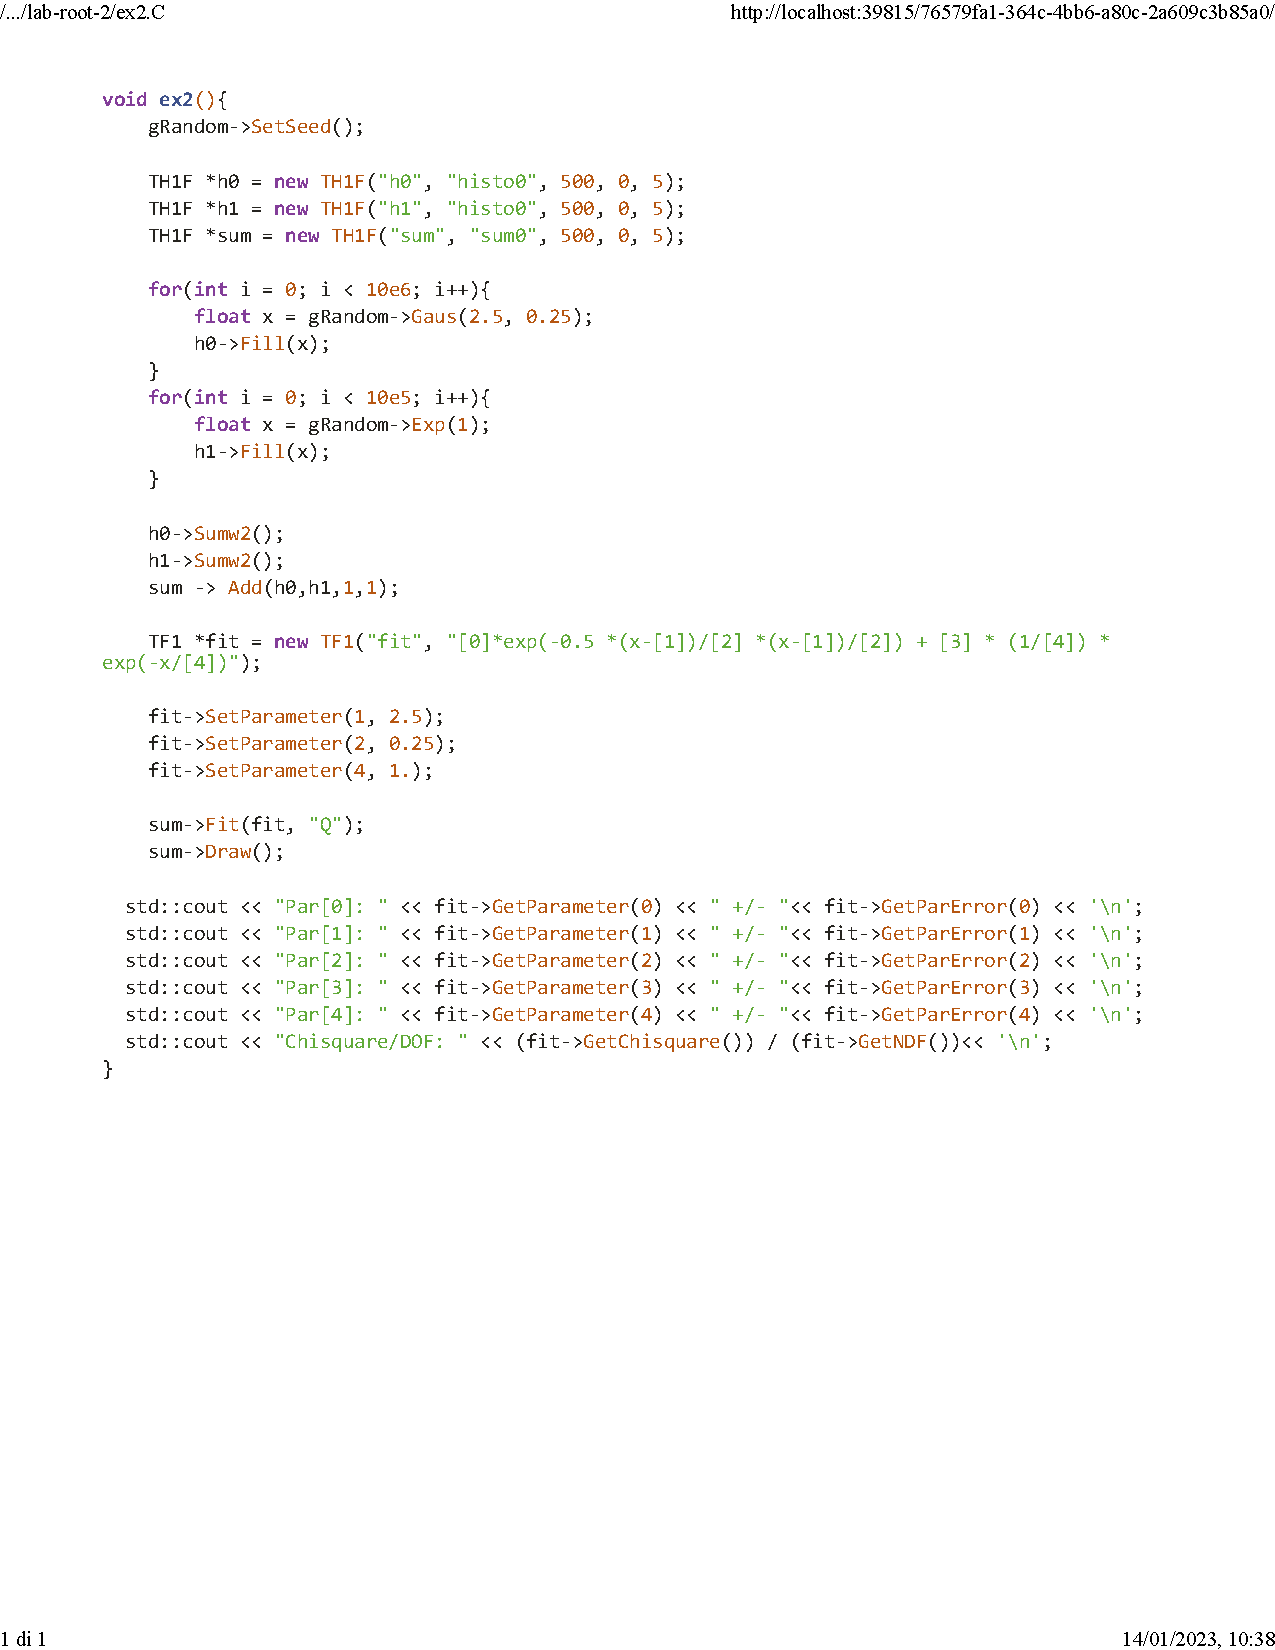
\includegraphics[width=1.\linewidth]{_..._lab-root-2_ex2.C}
	\caption{Fit di variabile generata casualmente secondo pdf con metodo di montecarlo.}
	\label{fig:6}
\end{figure}
\newpage
\subsection{Simulare effetto smearing}
Nelle misure reali, teoricamente distribuite gaussianamente, si osserva talvolta che la gaussiana non presenta un picco preciso ma un plateau di massimo non puntiforme, questo effetto si simula con lo "smearing" di una curva gaussiana generata mediante PRNG. In pratica, al posto di riempire l'istogramma con una distribuzione di media con un valore fissato, si usa una media a sua volta distribuita secondo una pdf uniforme. Di seguito è riportato un esempio di generazione gaussiana senza e con smearing\\\\
double media = 1.5;\\
for(int i = 0; i< 10e5; i++){\\
	h -> Fill(gRandom->Gaus(media, sigma))\\
}\\\\
double media = gRandom->Uniform(1, 2);\\
for(int i = 0; i< 10e5; i++){\\
	h -> Fill(gRandom->Gaus(media, sigma))\\
}\\\\
\newpage
\begin{figure}[h!]
	\centering
	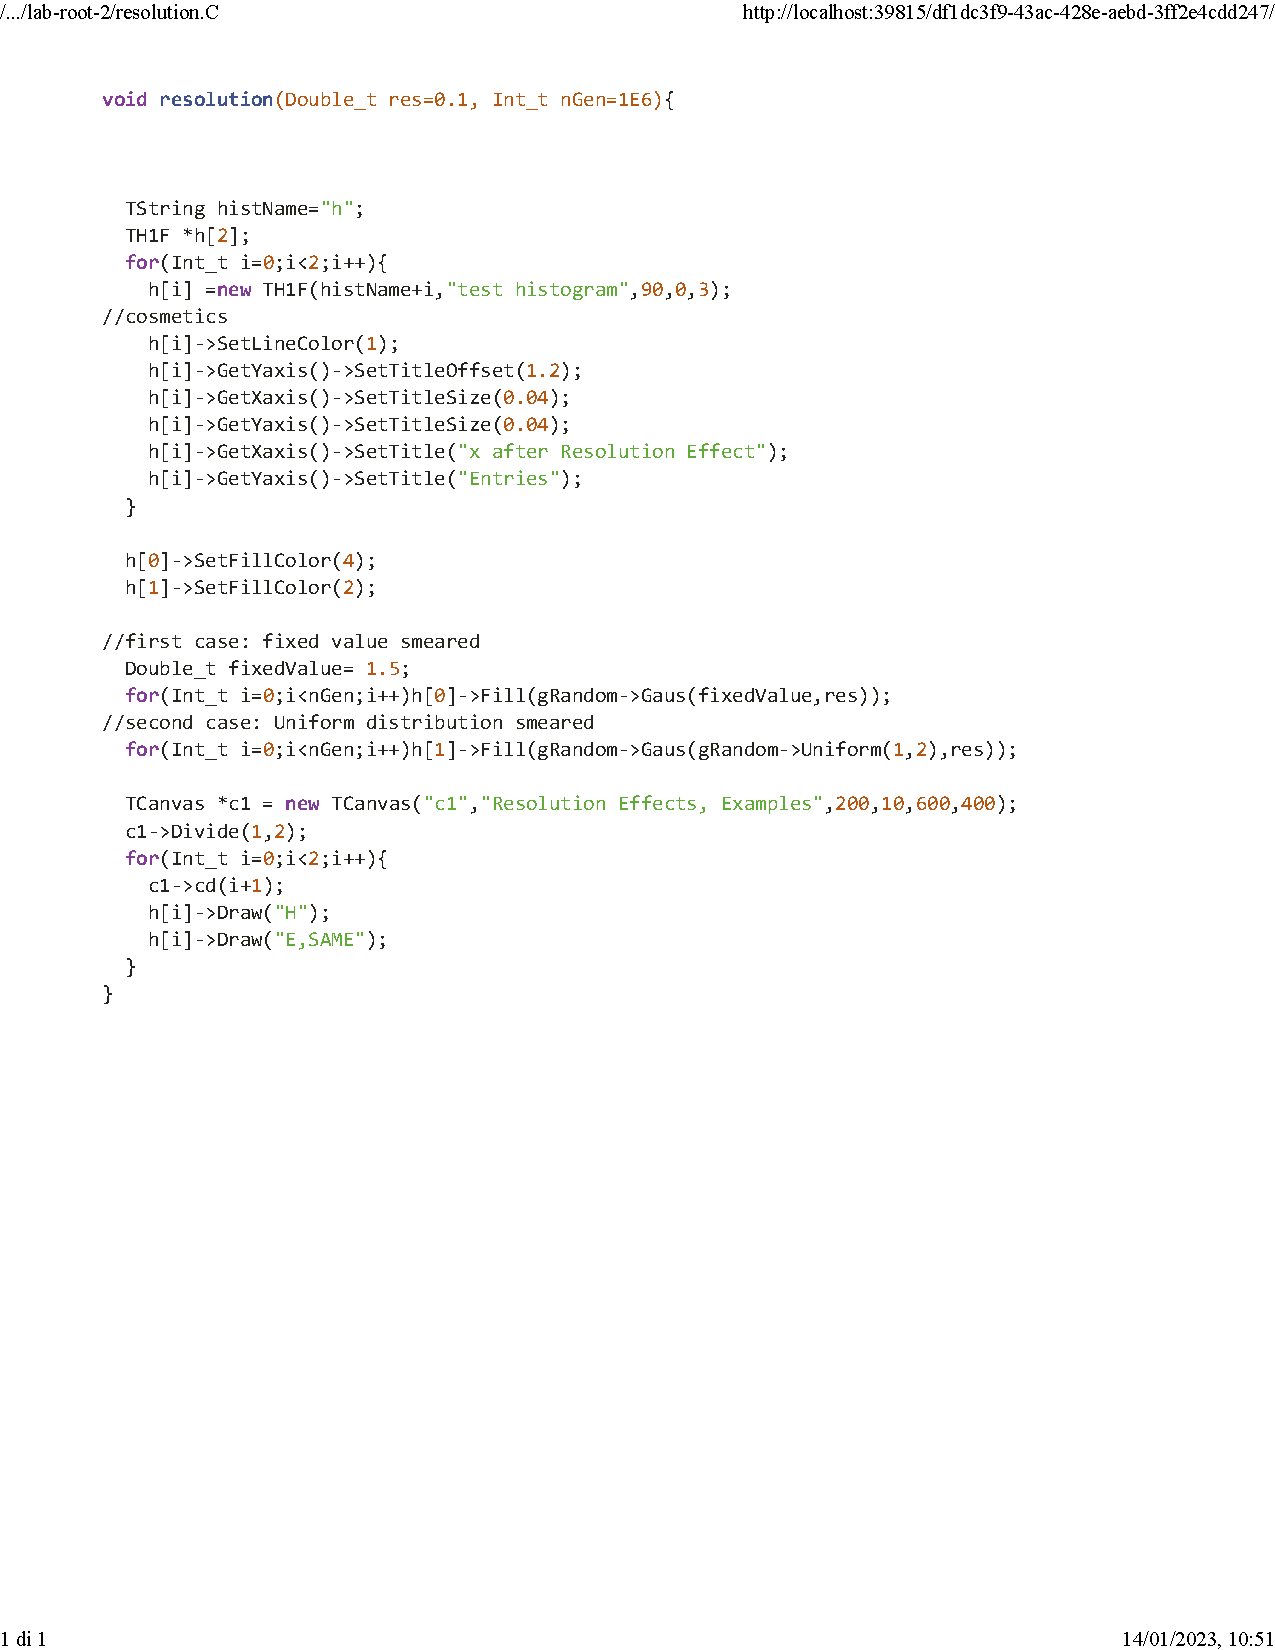
\includegraphics[width=1.\linewidth]{_..._lab-root-2_resolution.C}
	\caption{Esempio di simulazione di effetto smearing}
\end{figure}
\newpage 
\subsection{Simulare efficienza}
Gli strumenti di rilevazione sono sempre caratterizzati da un'efficienza, espressa in percentuale e solitamente indicata con la lettera $\varepsilon$, che esprime l'efficienza con la quale vengono rilevati gli eventi (efficienza del 70\% equivale a dire che su 10 eventi reali ne rivela 7 in media). L'efficienza può essere costante, come nell'esempio appena fatto, o può seguire l'andamento di una funzione.\\
Per simulare un'acquisizione dati di una variabile distribuita secondo una pdf, tenedo conto dell'efficienza dello strumento (che ora consideriamo costante) bisogna 
\begin{itemize}
	\item Generare la variabile x distribuita casualmente secondo una pdf con una PRNG ed inserira in un istogramma (contenente gli eventi reali)
	\item Generare una variabile y distribuita uniformemente tra 0 ed 1
	\item Riempire un istogramma con i valori x solo se y è minore o uguale dell'efficienza richiesta\\\\
	if(y<$\varepsilon$) h->Fill(x);\\
	\item Infine, per ottenere l'istogramma dell'efficienza, dividere l'istogramma delle acquisizioni tenendo conto dell'efficienza con quello dei valori reali.
\end{itemize}
Se l'efficienza è funzione della variabile x ($\varepsilon(x)$), bisogna definire la funzione che segue l'efficienza ed inserire la x nell'istogramma solo se la y generata casualmente con distribuzione uniforme tra 0 e 1 è minore della funzione $\varepsilon(x)$, valutata nello specifico x. Per valutare la funzione si usa il metodo Eval.\\\\
 TF1 *eff = new TF1("eff", "$\varepsilon(x)$", \(x_min\), \(x_max\));\\
 if(y< eff->Eval(x)) h->Fill(x);\\\\
Si ricordi di dividere infine l'istogramma che tiene conto dell'efficienza con quello dei valori reali generati per ottenere un'istogramma dell'efficienza.\\
\'E frequente che l'efficienza segua la distribuzione cumulativa della gaussiana normale standard, detta error function, che su ROOT è implementata come TMath::Erf(x). Erf prende come parametro una variabile distribuita normalmente, per normalizzare il valore di una distribuzione gaussiana di media $\mu$ e deviazione standard $\sigma$ si usa
\[\frac{x-\mu}{\sigma}\]
Per definire la funzione Erf che normalizzi automaticamente la variabile ed usarla come efficienza bisogna definirla all'esterno della macro (usando la sintassi di C++) e poi inizializzarla all'interno di una funzione nella macro (come visto nella sezione sull'inizializzazione di funzioni). Le variabili di Erf vanno settate con il metodo SetParameter.\\\\\\
double effErf(double* x, double* p) \{\\
	//p[0]==media\\
	//p[1]==sigma\\
	//p[2]==valore di saturazione\\
	//offset 1 e fattore 1/2 per riscalare Erf in [0,1]\\
	
	return (TMath::Erf(  ( x[0] - p[0] ) / p[1] ) +1) / 2. * p[2];\\
\}
\newpage
\begin{figure}[h!]
	\centering
	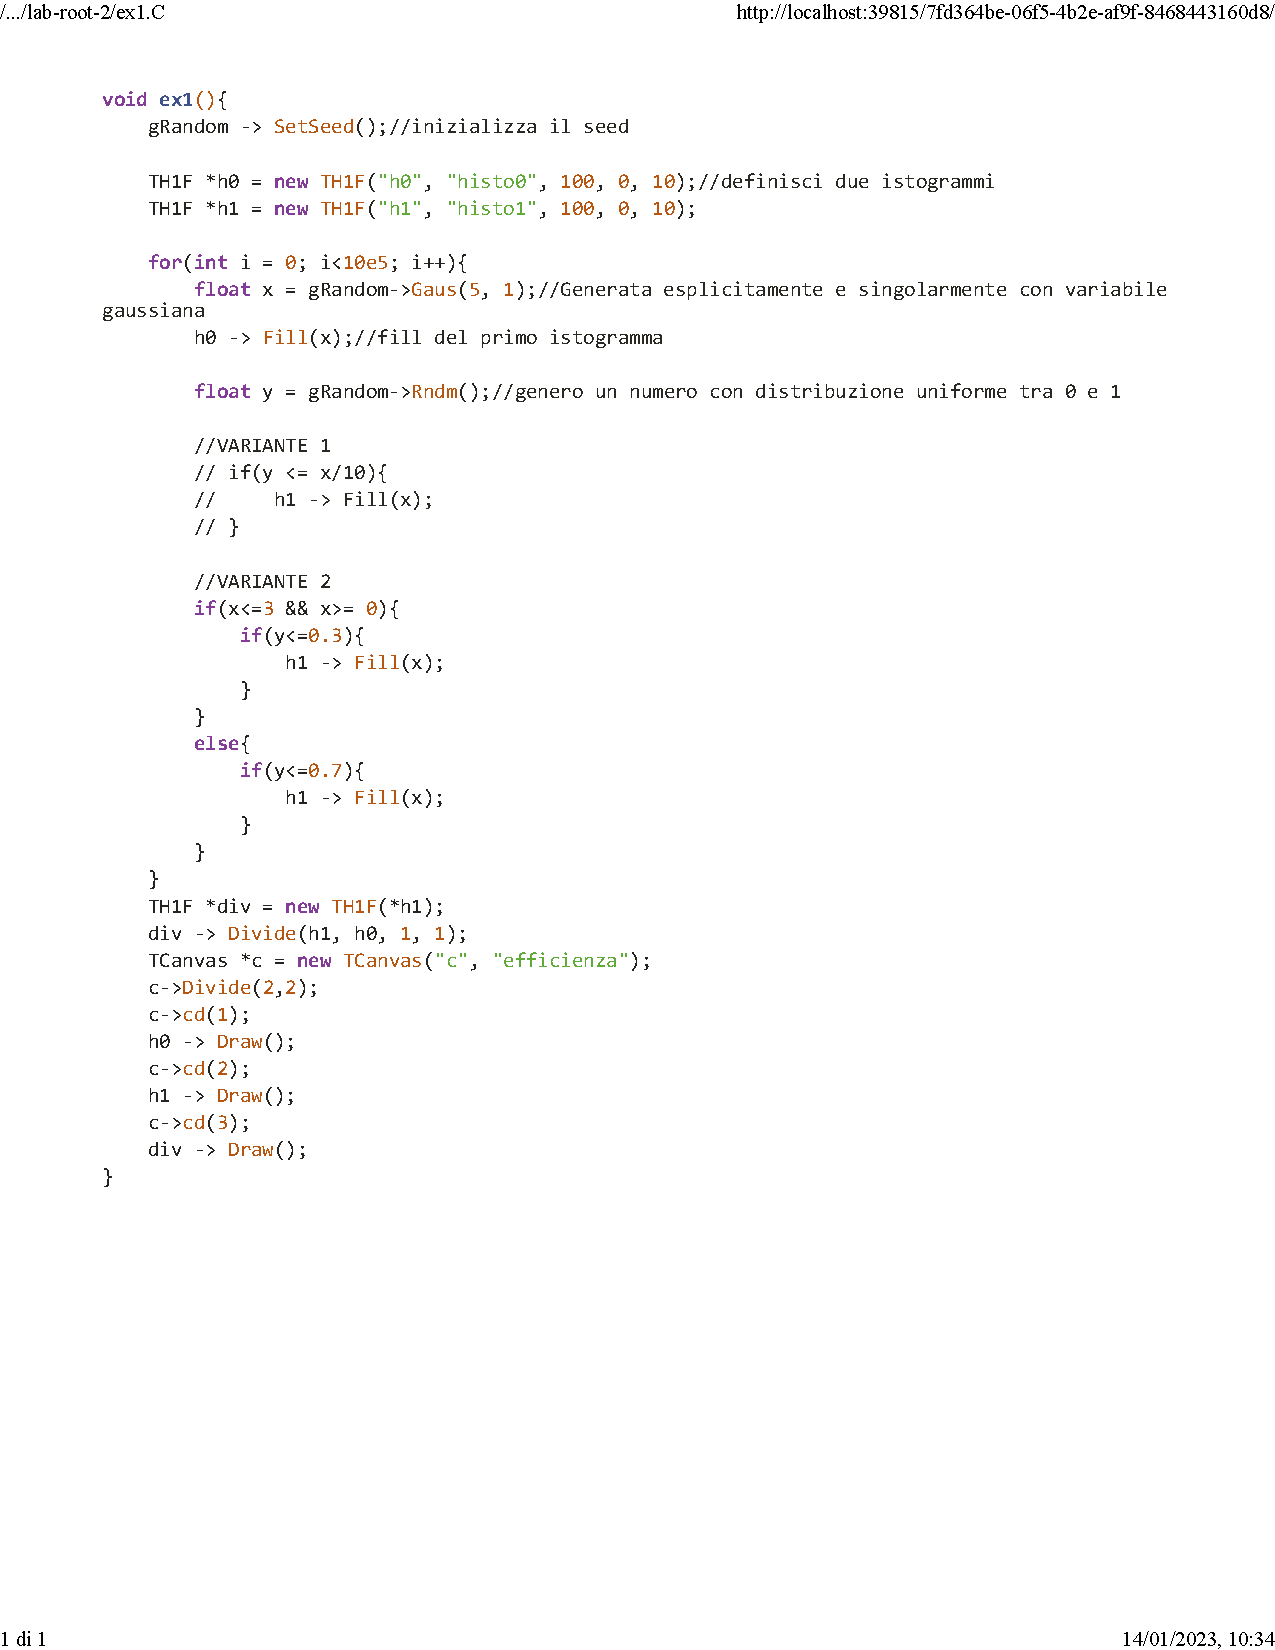
\includegraphics[width=1.\linewidth]{_..._lab-root-2_ex1.C}
	\caption{}
	\label{fig:4}
\end{figure}
\newpage
\begin{figure}[h!]
	\centering
	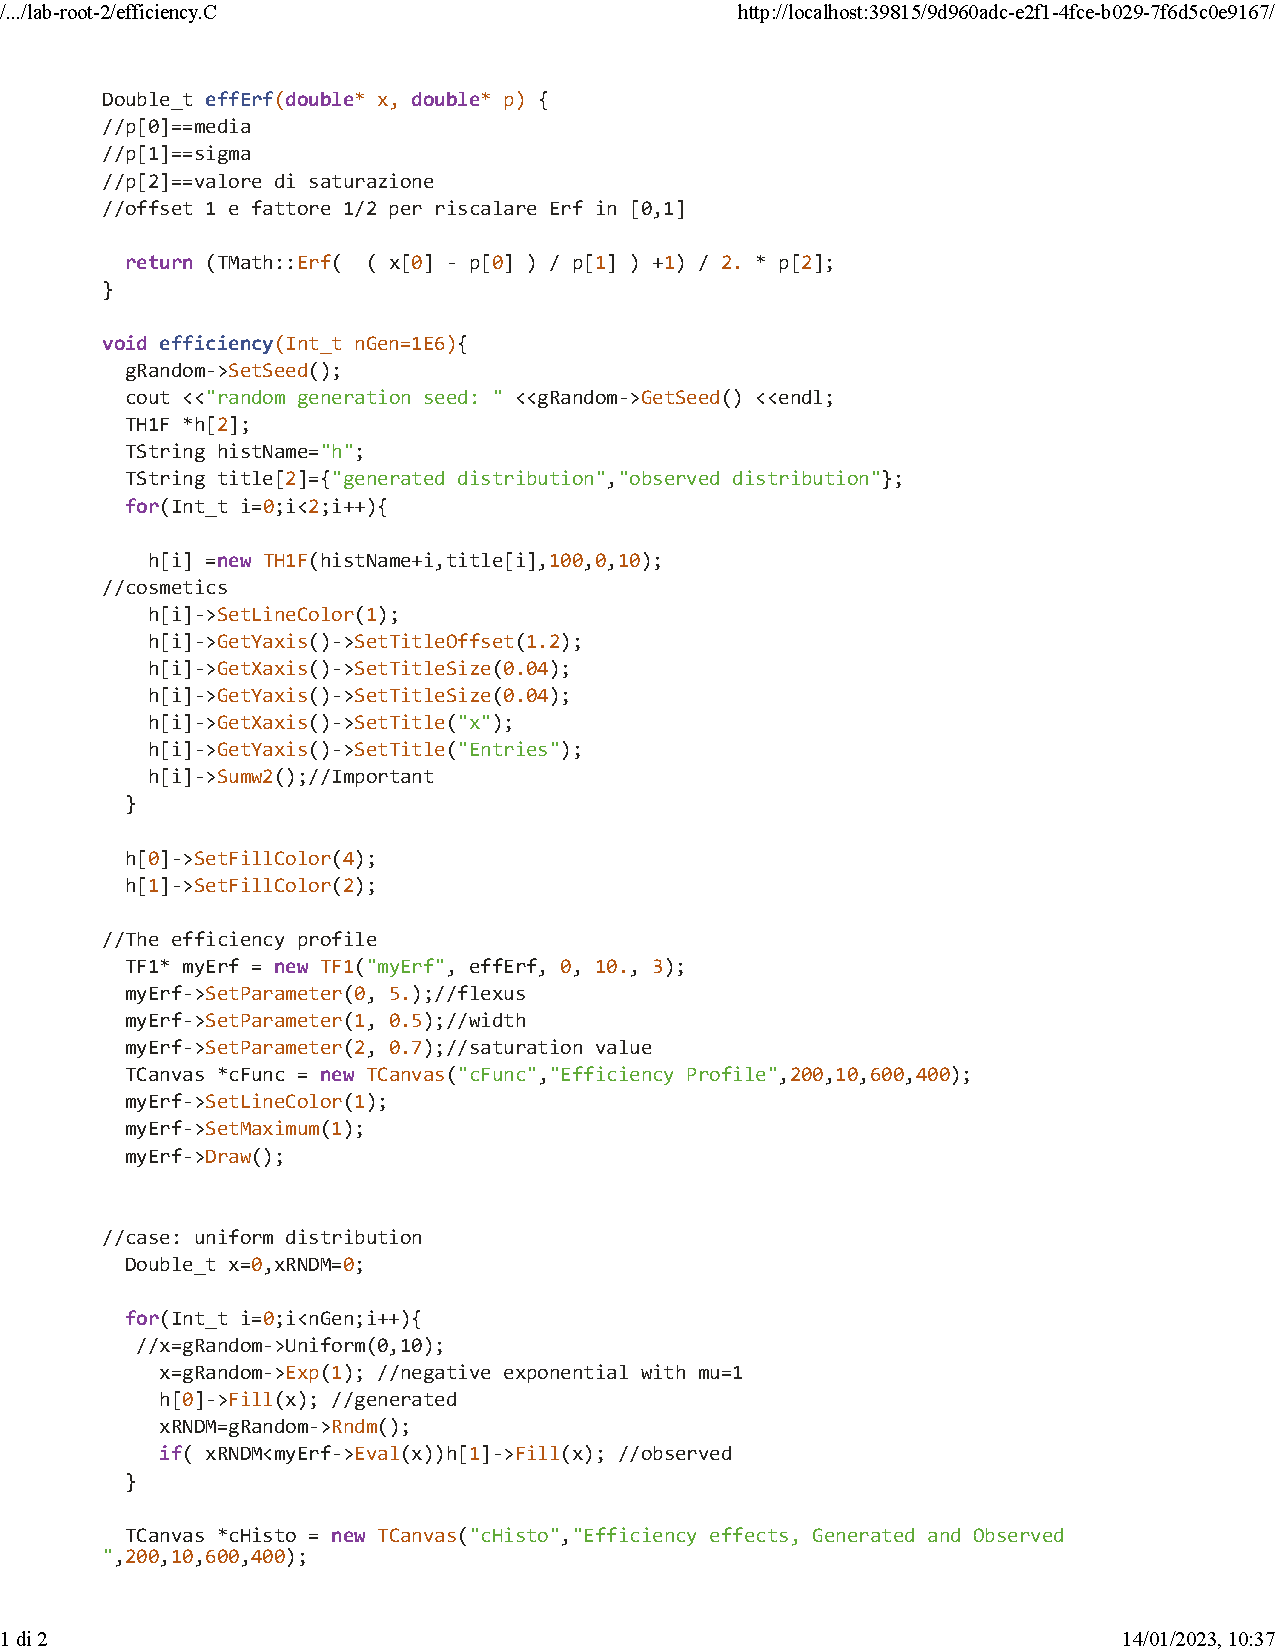
\includegraphics[width=1.\linewidth]{_..._lab-root-2_efficiency.C}
	\caption{}
	\label{fig:5}
\end{figure}
\newpage
\begin{figure}[h!]
	\centering
	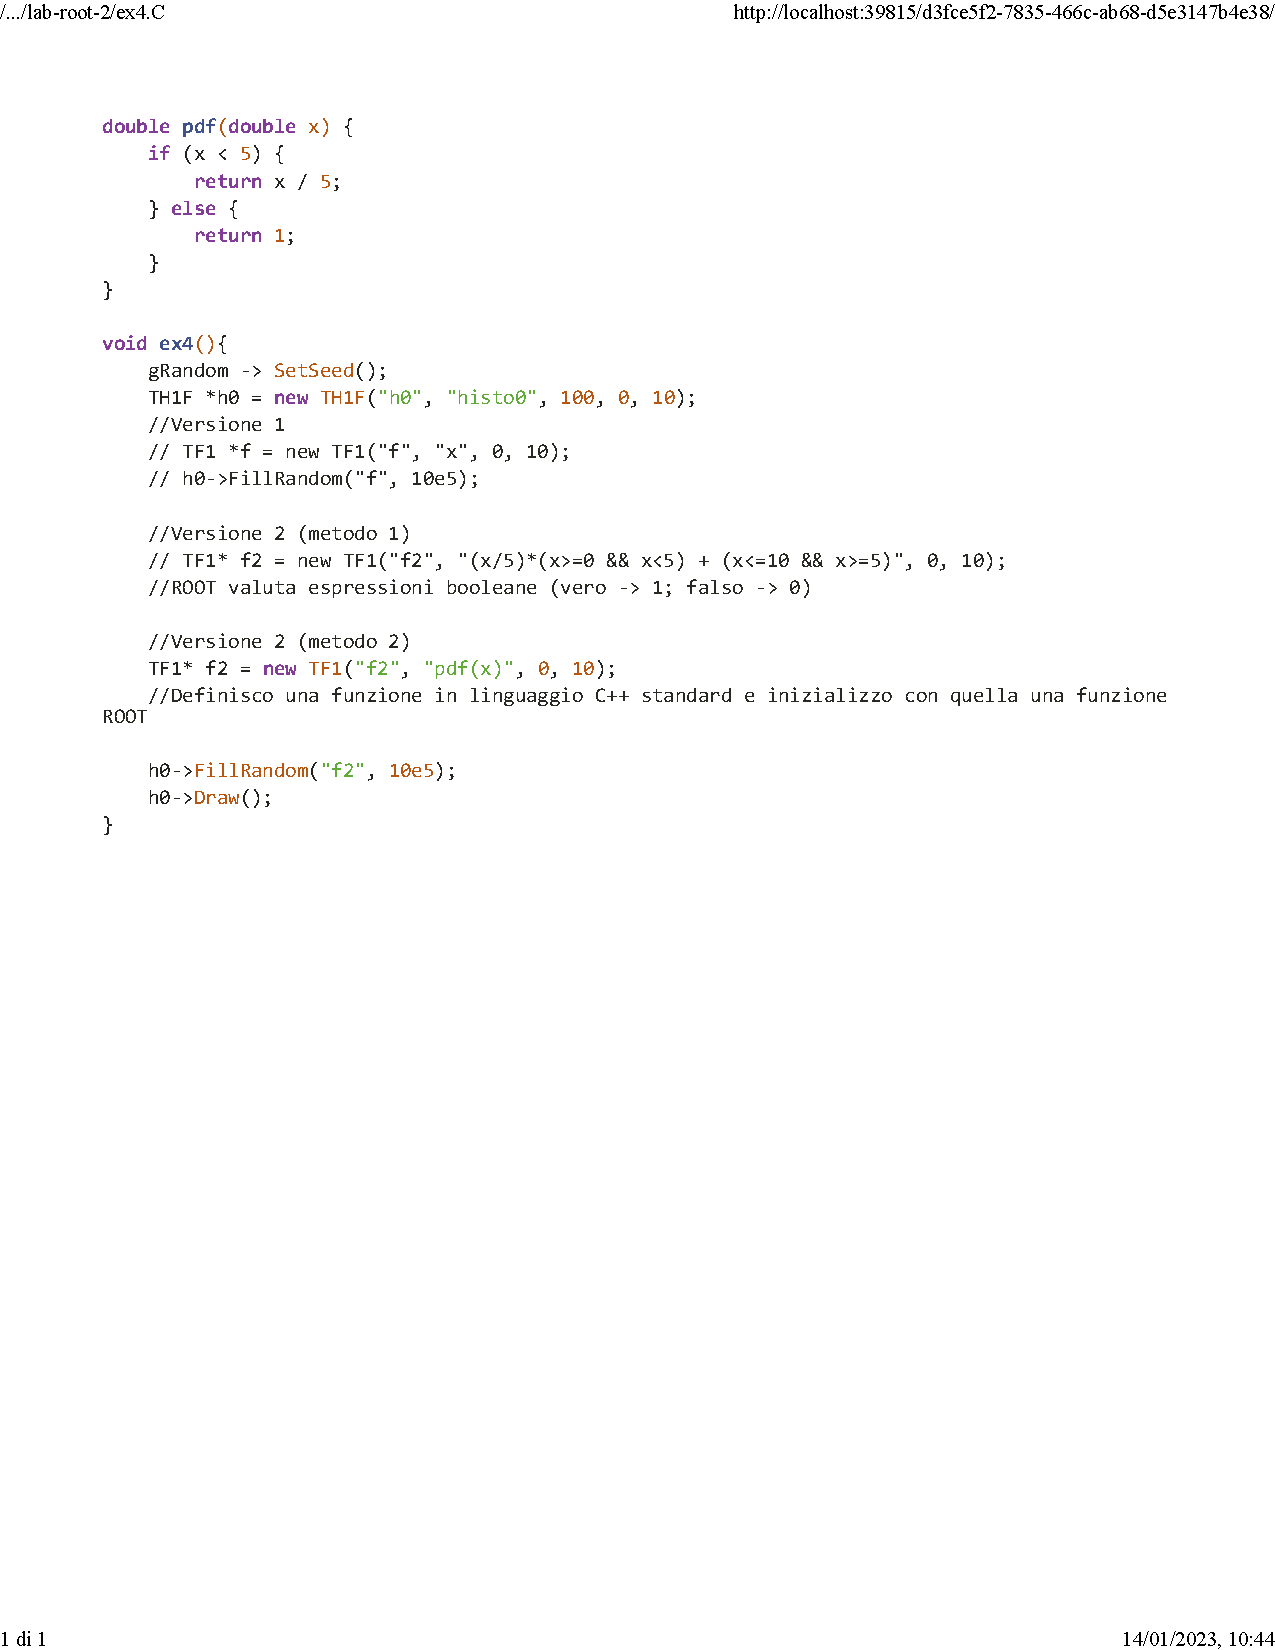
\includegraphics[width=1.\linewidth]{_..._lab-root-2_ex4.C}
	\caption{Simulazione di efficienza con funzione definita a tratti}
\end{figure}
\newpage
\section{Benchmark}
Il benchmark è un metodo per valutare la performance di una macro/programma di ROOT; esiste l'oggetto nativo di ROOT TBenchmark adatto allo scopo.\\
Innanzitutto bisogna creare l'oggetto TBenchmark, che come per gRandom deve essere istanziato una volta sola.\\\\
TBenchmark *b = new TBenchmark();\\\\
In seguito possiamo usare i 4 seguenti metodi
\begin{itemize}
	\item Start: comincia il conteggio del tempo, bisogna assegnare un nome\\\\
		b->Start("nome");\\
	\item Stop: ferma il conteggio del benchmark (già iniziato) con lo stesso nome\\\\
		b->Stop("nome");\\
	\item Print: Effettua automaticamente la stampa a schermo del tempo misurato fino a quel momento, senza fermare il conteggio.
	\item Show: è una combinazione di Stop e Print\\\\
		b->Show("nome");
\end{itemize}
\newpage
\begin{figure}[h!]
	\centering
	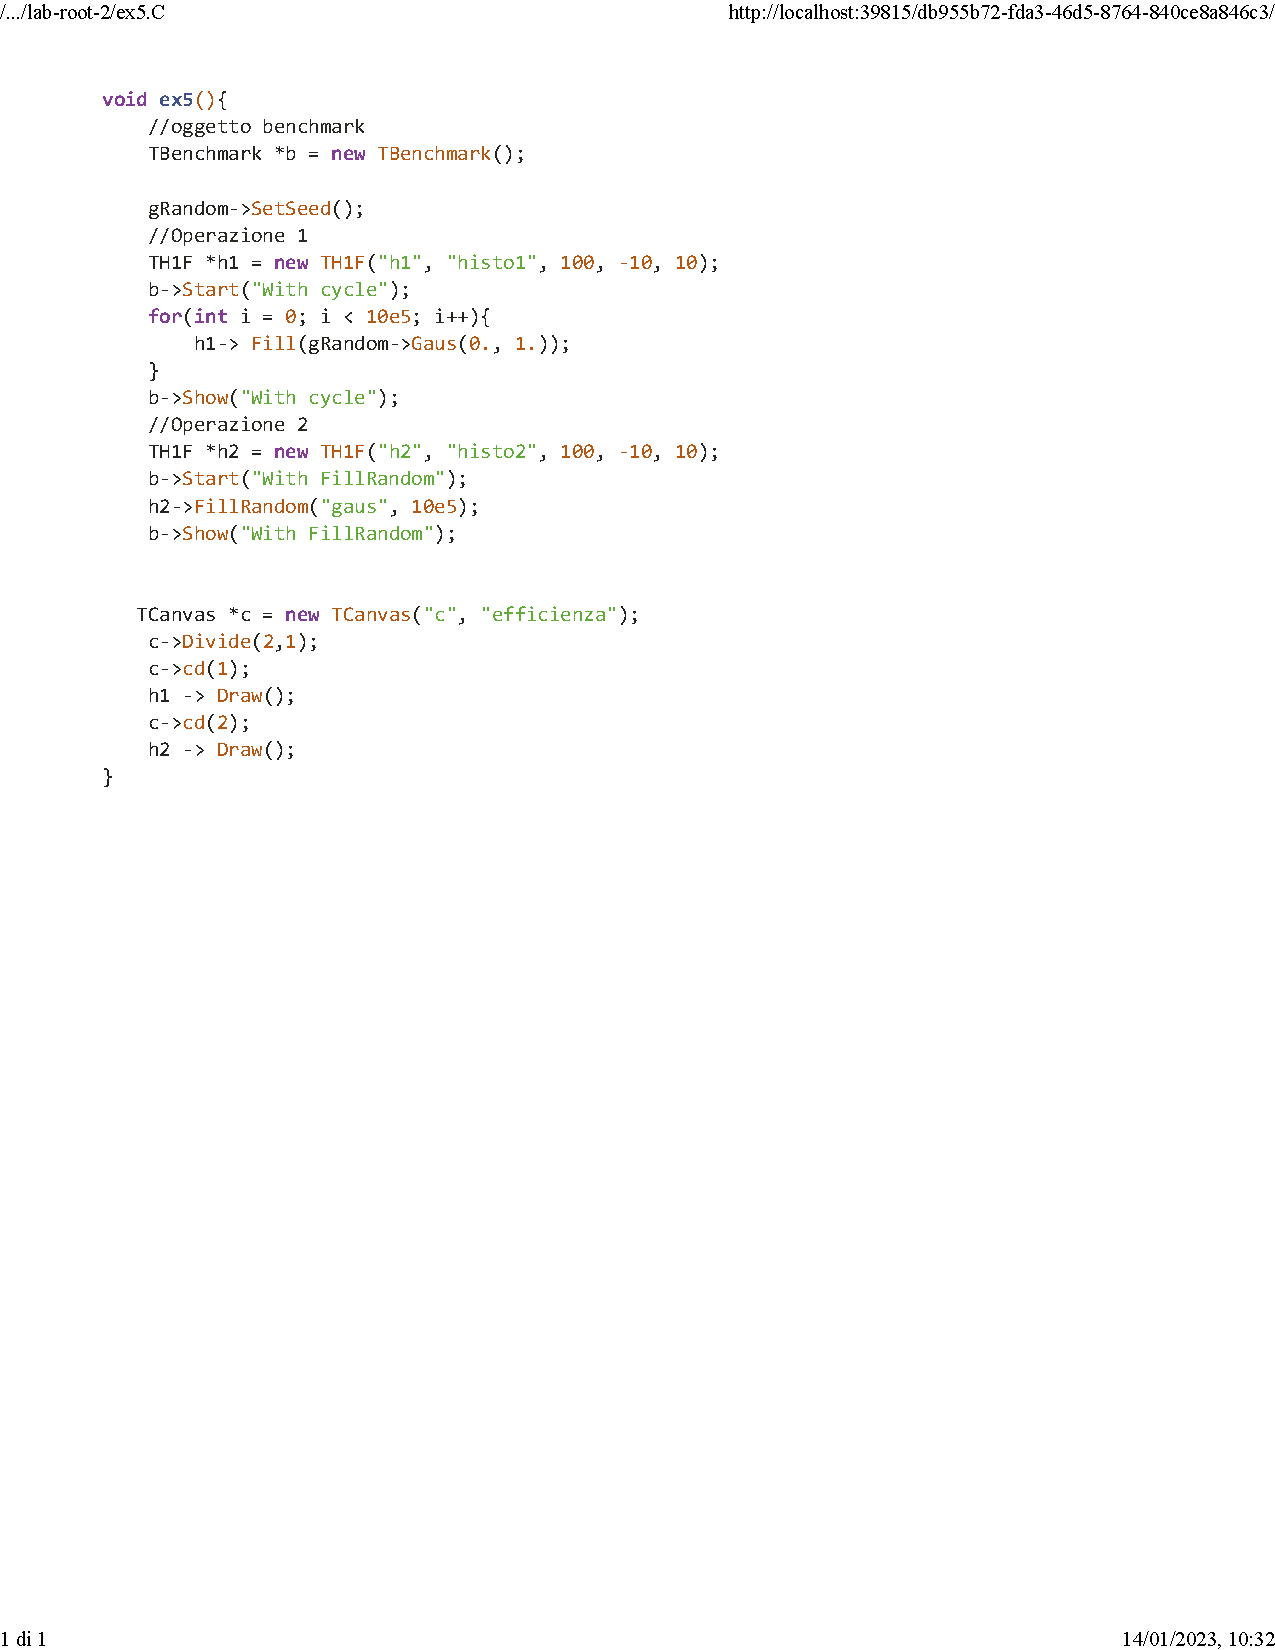
\includegraphics[width=1.\linewidth]{_..._lab-root-2_ex5.C}
	\caption{Esempio di utilizzo dei benchmark}
\end{figure}
\newpage
\section{Liste}
In ROOT esiste un oggetto simile alle liste della standard library: le TList. Queste non è altro che un container che può contenere oggetti eterogenei, a patto che derivino tutti da TObject (classe madre di tutti gli oggetti di ROOT). Per inizializzare una TList la sintassi è:\\\\
TList * list= new TList();\\\\
Per aggiungervi un'oggetto:\\\\
list->Add(obj);\\\\
Per accedere all'elemento i-esimo:\\\\
list->At(i);\\\\
Per stampare a schermo (testo) il contenuto della TList:\\\\
list->Print();\\\\
Infine, il metodo InheritsFrom("Tipo dell'oggetto") serve a controllare se un'oggetto è di un certo tipo, ad esempio può essere usato come condizione di un if:\\\\
if(!testList->At(i)->InheritsFrom("TH2")){\\
	testList->At(i)->Draw("H");\\
}\\\\
\section{Alberi}
Un tree è una struttura dati organizzata in "branches" che possono essere visti come cartelle all'interno dei quali si salvano dati correlati fra loro (che ad esempio è probabile vengano usati insieme), per convenzione ogni branch contiene sottostrutture dette leaves, ciascune delle quali corrisponde ad un tipo di dato.
\subsection{Creare e riempire un Tree}
Per usare un Tree innanzitutto bisogna inizializzare un file\\\\
TFile *F = new TFile("nome\_file.root", RECREATE);\\\\
 in seguito, oggetto di tipo Tree si inizializza con la seguente sintassi \\\\
TTree *t = new TTree("t, "titolo");\\\\
Per creare i branches si usa il metodo Branch\\\\
double x;
t -> ("x", \&x, "x/F");\\
Per riempire il tree si usail metodo Fill che riempie automaticamente il branch corretto. \\\\
t->Fill();\\\\
Infine si scrive il tree sul file e si chiude il file.\\\\
t->Write()\\
F->Close()\\
\newpage
\begin{figure}[h!]
	\centering
	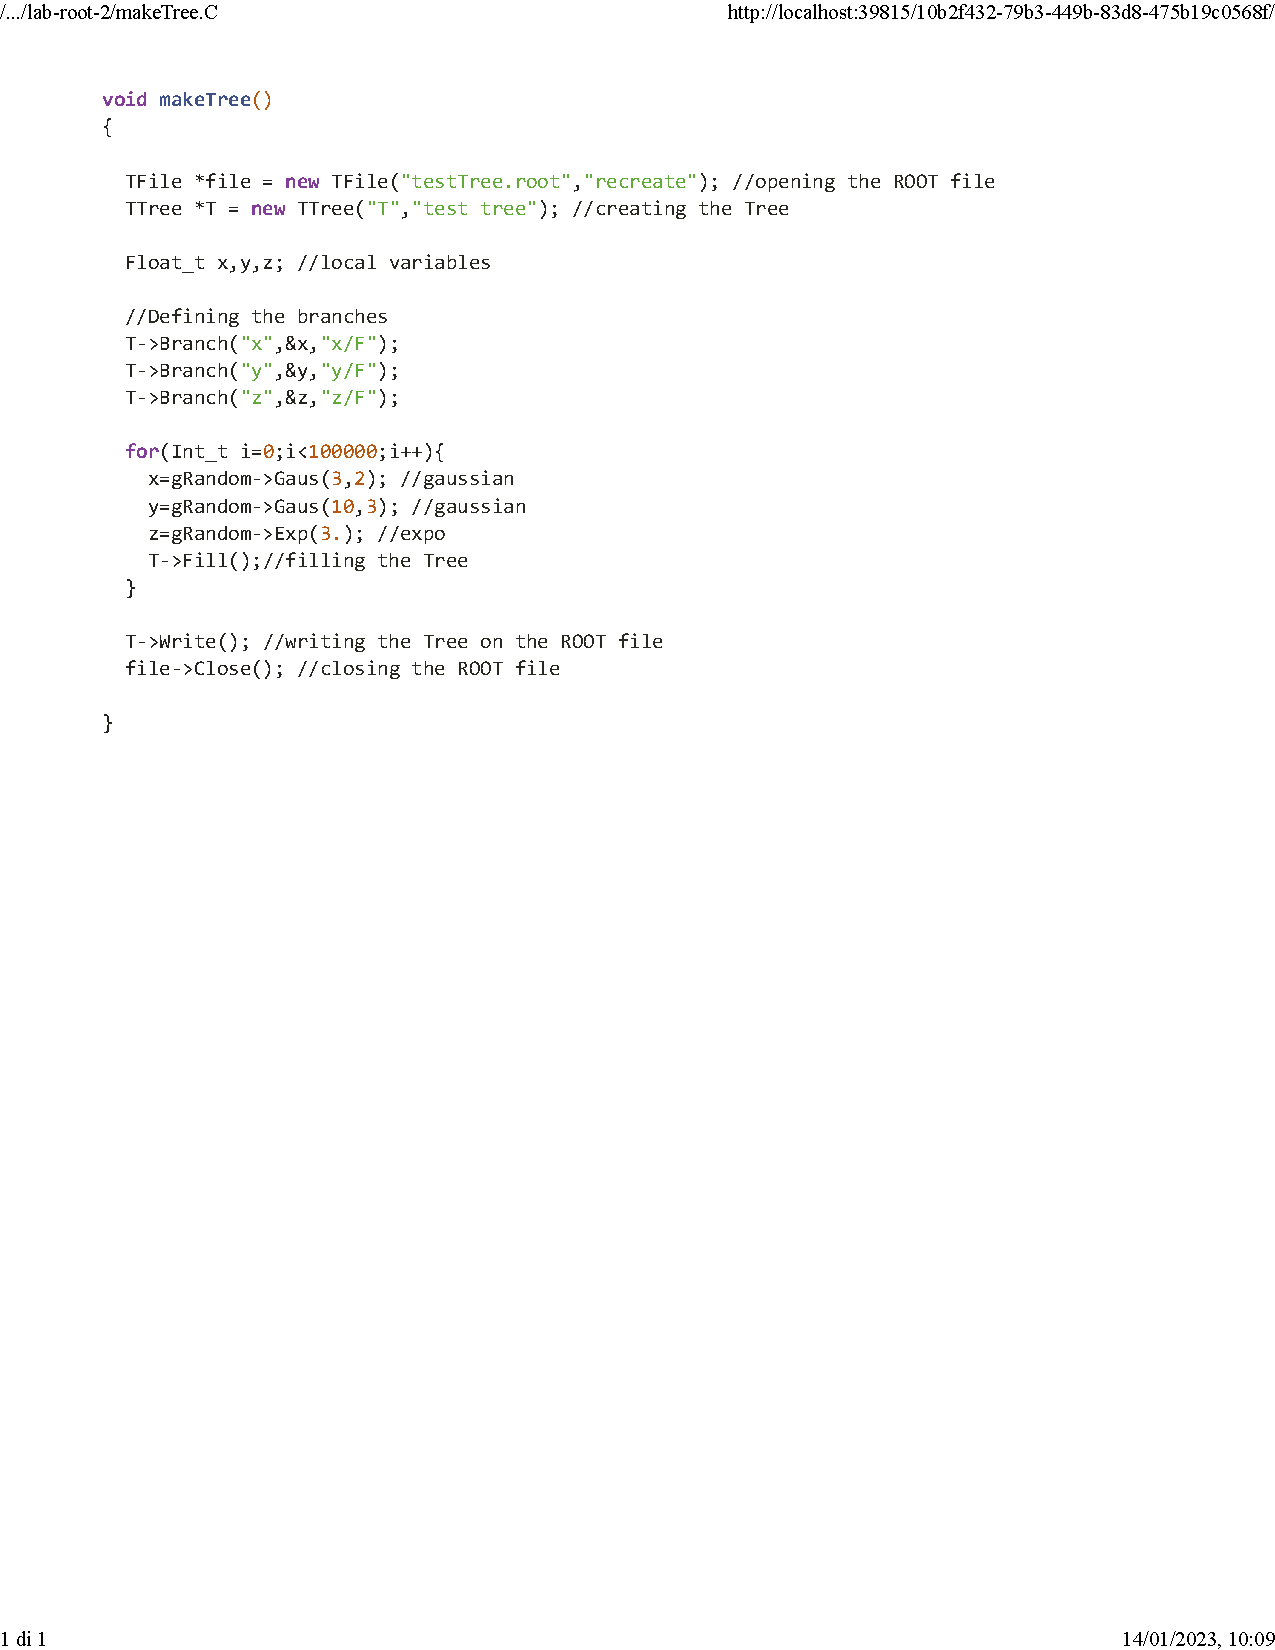
\includegraphics[width=1.\linewidth]{_..._lab-root-2_makeTree.C}
	\caption{}
	\label{fig:1}
\end{figure}
\newpage
\subsection{Analisi dati}
Una volta inizializzato e riempito l'albero possiamo passare alla fase di analisi dei dati salvati nell'albero. Innanzitutto per accedere al tree (creato in un altro file)  dal file di analisi dati, bisogna aprire il file precedente e recuperare il Tree\\\\
TFile *file = new TFile("test.root");\\
TTree * Tout= (TTree*)file->Get("T");\\
Per stampare a schermo le variabili contenute nel Tree si usa il metodo Print\\\\
Tout->Print();\\\\
Per graficare una variabile, ad esempio x (con nome binnaggio e range automatico):\\\\
Tout->Draw(“x”);\\\\
Per riempire e disegnare un istogramma user-defined con una variabile di un tree si usa l'operatore >> (dove x è il nome del branch):\\\\
TH1F *h 1= new TH1F("h1","hist from tree",50,-4, 4);\\
Tout->Draw("x>>h1");\\\\
\'E inoltre possibile imporre condizioni sulle variabili con un'opzione di Draw (che accetta operatori logici di C++)\\\\
Tout->Draw("x”,”y>0 \&\& x<10”);\\\\
Si possono disegnare anche grafici bi dimensionali e tridimensionali che correlano set di dati contenuti in diversi branches:\\\\
T->Draw(“y:x”);\\
T->Draw(“z:y:x”);\\
\newpage
\begin{figure}[h!]
	\centering
	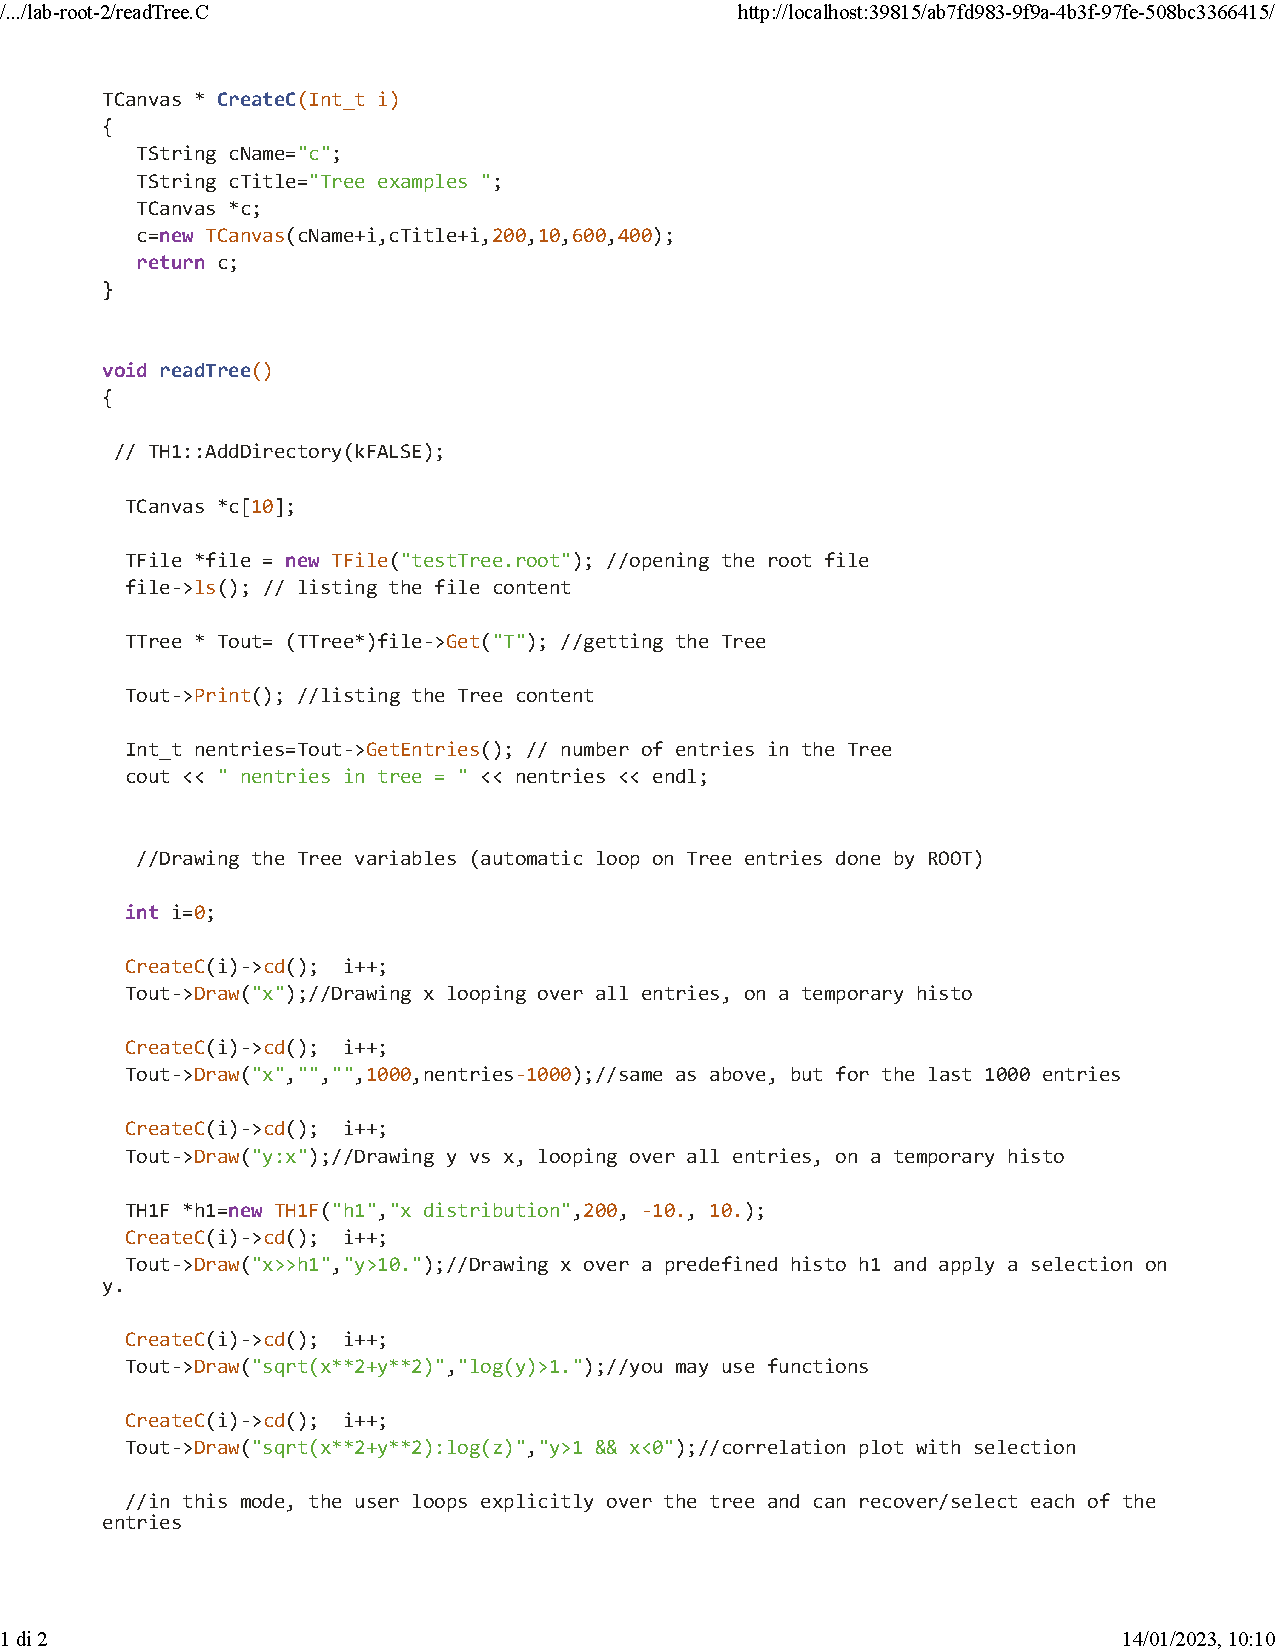
\includegraphics[width=1.\linewidth]{_..._lab-root-2_readTree.C}
	\caption{}
	\label{fig:2}
\end{figure}
\end{document}